% ---------------------------------------------------------------------------
% AVA-I - Proposta de Trabalho de Conclusão (LaTeX)
% Compilar: pdflatex tcc -> bibtex tcc -> pdflatex tcc -> pdflatex tcc
% Observação: os elementos pré-textuais (capa, folha de rosto) devem vir do
% template oficial da PUCRS (Moodle). Este arquivo traz o corpo do texto,
% com as citações ancoradas no .bib (tcc-bib.bib).
% ---------------------------------------------------------------------------
\documentclass[12pt,a4paper]{article}

\usepackage[utf8]{inputenc}
\usepackage[T1]{fontenc}
\usepackage[brazilian]{babel}
\usepackage[margin=2.5cm]{geometry}
\usepackage{setspace}
\usepackage{amsmath}
\usepackage{booktabs}
\usepackage{array}
\usepackage{enumitem}
\usepackage[hidelinks]{hyperref}
\usepackage{graphicx}
\graphicspath{{figuras/}}

\onehalfspacing
\setlength{\parindent}{1.25cm}
\setlength{\parskip}{0.2em}

\title{\textbf{Análise Comportamental e Avaliação Formativa:\\ Proposta de um Ambiente Virtual de Aprendizagem Inteligente}}
\author{Nicolas Pietro Moura da Silva \\ Orientador: Prof. Otávio Parraga}
\date{Porto Alegre, 2026}

\begin{document}
\maketitle

% ===========================================================================
\begin{abstract}
\noindent O ensino remoto e híbrido tornou os Ambientes Virtuais de Aprendizagem (AVAs) parte da rotina de estudo \cite{HBF19,Bat19}, mas o estudo autônomo nesses ambientes esbarra em dois problemas recorrentes: a atenção se dispersa durante a leitura \cite{KDB17} e falta um mecanismo que verifique, na hora, se o conteúdo foi compreendido \cite{DDD17}. Este trabalho propõe um AVA inteligente com três módulos. O primeiro recebe o material do professor e gera, automaticamente, questões formativas ancoradas nesse material, usando \emph{Retrieval-Augmented Generation} (RAG), em que um modelo de linguagem responde guiado por trechos recuperados do próprio conteúdo, em vez de ``inventar'' a resposta \cite{LPP20,GXG23}. O segundo estima, localmente no navegador do estudante, indicadores de engajamento visual a partir da câmera, combinando o estado dos olhos e a direção da cabeça com a detecção de \emph{smartphones}. O terceiro entrega ao professor um painel analítico que cruza esses indicadores com o desempenho nas questões. Quando o computador do estudante não consegue rodar o modelo de detecção de objetos, o sistema segue apenas com os indicadores mais leves, comportamento que chamamos de degradação graciosa, ou seja, o recurso pesado é desligado sem derrubar a aplicação. A proposta detalha o problema, o referencial teórico, a arquitetura, a metodologia e o plano de avaliação, este último condicionado à aprovação do Comitê de Ética em Pesquisa.

\vspace{0.5em}
\noindent\textbf{Palavras-chave:} ambiente virtual de aprendizagem; modelos de linguagem; geração aumentada por recuperação; visão computacional; engajamento; avaliação formativa; LGPD.
\end{abstract}

% ===========================================================================
\section{Introdução}

A transformação digital do ensino, acelerada pela pandemia de COVID-19, tornou os Ambientes Virtuais de Aprendizagem (AVAs) uma infraestrutura padrão na educação presencial, híbrida e remota \cite{HBF19,Bat19}. Esse movimento ampliou o acesso ao material didático, mas transferiu ao estudante uma carga maior de autorregulação: cabe a ele decidir quando, como e com que profundidade estudar. Ao mesmo tempo, técnicas de Inteligência Artificial (IA), em especial de Processamento de Linguagem Natural (PLN) e de Visão Computacional (VC), passaram a operar dentro de plataformas educacionais, apoiando a personalização do ensino e o acompanhamento do engajamento \cite{Van11,HBF19}.

Mesmo com AVAs maduros, o estudo autônomo enfrenta dois gargalos. O primeiro é a dispersão da atenção: o estudante alterna constantemente entre o material e estímulos externos, sobretudo o celular, o que eleva a carga cognitiva e prejudica a aprendizagem \cite{KDB17,Bat19}. O segundo é a passividade do material: o aluno lê PDFs e \emph{slides} sem nenhum ponto de verificação imediato, o que alimenta uma sensação de domínio que nem sempre corresponde à retenção real \cite{DDD17}.

Do lado do professor, somam-se outros dois problemas. Produzir avaliação formativa contínua não escala: extrair manualmente os conceitos-chave de cada material para gerar exercícios é trabalhoso e raramente acompanha o ritmo do semestre. E falta visibilidade sobre o processo: o professor recebe as notas, mas não enxerga onde a turma se dispersou nem qual material gerou mais dificuldade. Os Sistemas de Tutoria Inteligente (ITS) clássicos já mostraram que a tutoria assistida por computador pode produzir ganhos de aprendizagem próximos aos da tutoria humana individual \cite{Van11}, mas dependiam de regras escritas à mão, o que limitava sua escala. Os modelos de linguagem de grande porte (LLMs) \cite{BMR20,ZZL23} e a arquitetura de RAG \cite{LPP20,GXG23} mudam esse cenário: hoje é viável gerar perguntas formativas ancoradas no material do próprio professor, com risco controlado de erro, algo inviável nos tutores simbólicos da década passada.

Diante disso, este trabalho propõe um Ambiente Virtual de Aprendizagem Inteligente que reúne, numa única plataforma, a geração automática de avaliações formativas, a medição local de engajamento e um painel para o professor. As seções seguintes detalham os objetivos; o Capítulo~\ref{sec:ref} aprofunda os fundamentos que sustentam cada uma dessas escolhas.

\subsection{Objetivos}

O objetivo geral é propor, projetar e avaliar um Ambiente Virtual de Aprendizagem Inteligente que integre (i) a geração automática de avaliações formativas, por RAG, sobre o material do professor; (ii) a inferência local de indicadores de engajamento visual no navegador do estudante; e (iii) um painel analítico que permita ao professor cruzar engajamento e desempenho.

São objetivos específicos:
\begin{enumerate}[leftmargin=*]
  \item Revisar o estado atual sobre ITS, RAG aplicada à educação e medição automática de engajamento por VC.
  \item Especificar a arquitetura da plataforma, discutindo de forma explícita as restrições de \emph{hardware} no cliente e os requisitos de privacidade impostos pela Lei Geral de Proteção de Dados (LGPD) \cite{Bra18}.
  \item Implementar uma Prova de Conceito (PoC) funcional dos três módulos.
  \item Validar a PoC com estudantes voluntários, mediante aprovação do Comitê de Ética em Pesquisa (CEP) da PUCRS, usando métodos estatísticos adequados ao tamanho da amostra.
\end{enumerate}

% ===========================================================================
\section{Referencial Teórico}\label{sec:ref}

Este capítulo aprofunda os fundamentos que sustentam a proposta. A Seção~\ref{sub:aten} trata da dispersão da atenção e do automonitoramento da aprendizagem. A Seção~\ref{sub:its} examina os Sistemas de Tutoria Inteligente, os LLMs e a arquitetura de RAG. A Seção~\ref{sub:vc} descreve como a visão computacional mede engajamento. A Seção~\ref{sub:priv} trata da privacidade e da conformidade com a LGPD.

\subsection{Dispersão da atenção e automonitoramento da aprendizagem}\label{sub:aten}

Estudar em ambientes digitais exige autorregulação, e a pesquisa mostra que essa autorregulação costuma ser superestimada. Kirschner e De Bruyckere \cite{KDB17} desmontam o mito do ``nativo digital'': a crença de que jovens conseguem alternar sem custo entre estudar e usar aplicativos não se sustenta; na prática, essa alternância contínua eleva a carga cognitiva e degrada o desempenho. Bates \cite{Bat19} descreve o \emph{cyber-slacking}, isto é, o uso oportunista do dispositivo para fins não acadêmicos durante o estudo, e seu efeito sobre a memória de trabalho. D'Mello, Dieterle e Duckworth \cite{DDD17} propõem um arcabouço para medir engajamento de forma automatizada, combinando sinais comportamentais (como postura e direção do olhar) com sinais afetivos.

Um conceito é central nesse debate: o automonitoramento da aprendizagem, ou seja, a capacidade do estudante de acompanhar e regular o próprio progresso. O problema da leitura passiva está justamente nesse ponto: sem retorno, o aluno não detecta a própria distração nem as lacunas de compreensão. A literatura converge para uma solução prática: inserir \emph{feedback} imediato e pontos de verificação ao longo do estudo ajuda o aluno a perceber e corrigir a dispersão antes que ela vire fracasso na avaliação \cite{DDD17,Van11}. Essa constatação motiva, na proposta, intercalar a leitura com perguntas formativas.

\subsection{Sistemas de Tutoria Inteligente, LLMs e RAG}\label{sub:its}

Sistemas de Tutoria Inteligente (ITS) ajustam o ritmo, a sequência e o conteúdo da instrução conforme o estado de conhecimento do aluno. A meta-análise de VanLehn \cite{Van11} é a referência clássica: ITS bem projetados, que interagem com o aluno em granularidade fina (passo a passo), alcançam ganhos de aprendizagem comparáveis aos da tutoria humana individual. Historicamente, porém, esses sistemas dependiam de bases de regras escritas e mantidas manualmente, o que tornava cara e lenta a sua expansão para novos conteúdos.

Os LLMs \cite{BMR20,ZZL23} alteraram esse quadro ao permitir gerar conteúdo pedagógico, inclusive perguntas, a partir de instruções em linguagem natural. Há, contudo, um risco conhecido: operados sem ancoragem em uma fonte confiável, esses modelos produzem alucinações, isto é, afirmações que soam plausíveis, mas são falsas. A arquitetura de \emph{Retrieval-Augmented Generation} (RAG), proposta por Lewis et al. \cite{LPP20} e sistematizada por Gao et al. \cite{GXG23}, reduz esse risco: antes de responder, o sistema recupera de uma base externa os trechos mais relevantes e os entrega ao modelo como contexto, fazendo a geração se apoiar no material de referência em vez da memória do modelo.

O fluxo de RAG funciona em duas etapas. Primeiro, o texto-fonte é dividido em fragmentos (\emph{chunks}) e convertido em vetores (\emph{embeddings}) que preservam a proximidade de significado entre trechos parecidos; esses vetores ficam guardados em um banco vetorial. Depois, na geração, a consulta também é convertida em vetor, os fragmentos mais próximos são recuperados, e o modelo produz a resposta condicionada a esse contexto \cite{GXG23}. Essa abordagem se encaixa bem no problema de gerar avaliações ancoradas em um material específico, pois nele a ``verdade de referência'' é um conjunto de documentos delimitado e conhecido, exatamente o material do professor.

\subsection{Medição visual de engajamento}\label{sub:vc}

A análise automática de engajamento por VC se apoia em dois sinais: o rastreamento do rosto do estudante e a detecção de objetos no seu ambiente.

Ferramentas de rastreamento facial permitem estimar a posição da cabeça e o estado dos olhos. O MediaPipe Face Mesh \cite{LTN19,KAGG19}, por exemplo, estima em tempo real centenas de pontos do rosto a partir de uma câmera comum, é leve o bastante para rodar no navegador e tem uso recorrente em estudos de engajamento educacional \cite{AK24,DD25}. Sobre esses pontos, calcula-se o \emph{Eye Aspect Ratio} (EAR), proposto por Soukupová e Cech \cite{SC16}, que resume em um único número o grau de abertura dos olhos e serve de base para detectores de piscada e de sonolência validados \cite{MdCMSL20}. Ao combinar o EAR com a direção da cabeça, infere-se, com confiabilidade razoável, se o estudante está olhando para a tela do material.

O segundo sinal é a presença de um \emph{smartphone} no campo da câmera, indício de \emph{cyber-slacking}. Para detectá-lo, emprega-se a família de modelos YOLO (\emph{You Only Look Once}) \cite{RDGF16}, na versão YOLOv8 \cite{JCQ23}, que oferece variantes ``nano'', pequenas o suficiente para inferência no navegador. Vale registrar uma limitação: a inferência do YOLO no navegador depende do \emph{hardware} do estudante e pode pesar em máquinas modestas \cite{JCQ23}. A proposta trata explicitamente essa restrição na Seção~\ref{sub:hw}, com um caminho de contingência.

\subsection{Privacidade, LGPD e processamento no cliente}\label{sub:priv}

O monitoramento por câmera em contexto educacional é sensível: o vídeo de um estudante é dado pessoal e, no caso de menores, dado pessoal de criança e adolescente, com proteção reforçada pela LGPD (Lei nº 13.709/2018) \cite{Bra18}. A literatura sobre IA educacional ética \cite{HBF19,UNE21} recomenda o princípio de \emph{privacy by design}, que consiste em projetar o sistema, desde o início, para coletar o mínimo e processar os dados o mais perto possível da origem, em vez de tratar a privacidade como política adicionada depois. Seguindo esse princípio, a proposta executa toda a visão computacional no próprio navegador do estudante: nenhum quadro de vídeo trafega pela rede, e o servidor recebe apenas métricas numéricas agregadas.

% ===========================================================================
\section{Proposta}

Este capítulo apresenta o sistema em nível conceitual. A discussão técnica detalhada está no Capítulo~\ref{sec:arq} (arquitetura) e no Capítulo~\ref{sec:met} (metodologia).

\subsection{Visão geral do sistema}

Propõe-se um Ambiente Virtual de Aprendizagem Inteligente (AVA-I), em formato de aplicação web, com três módulos integrados. As figuras desta seção apresentam a prova de conceito já implementada. A Figura~\ref{fig:lobby} mostra a tela inicial, com acesso aos três módulos.

\begin{figure}[htbp]
\centering
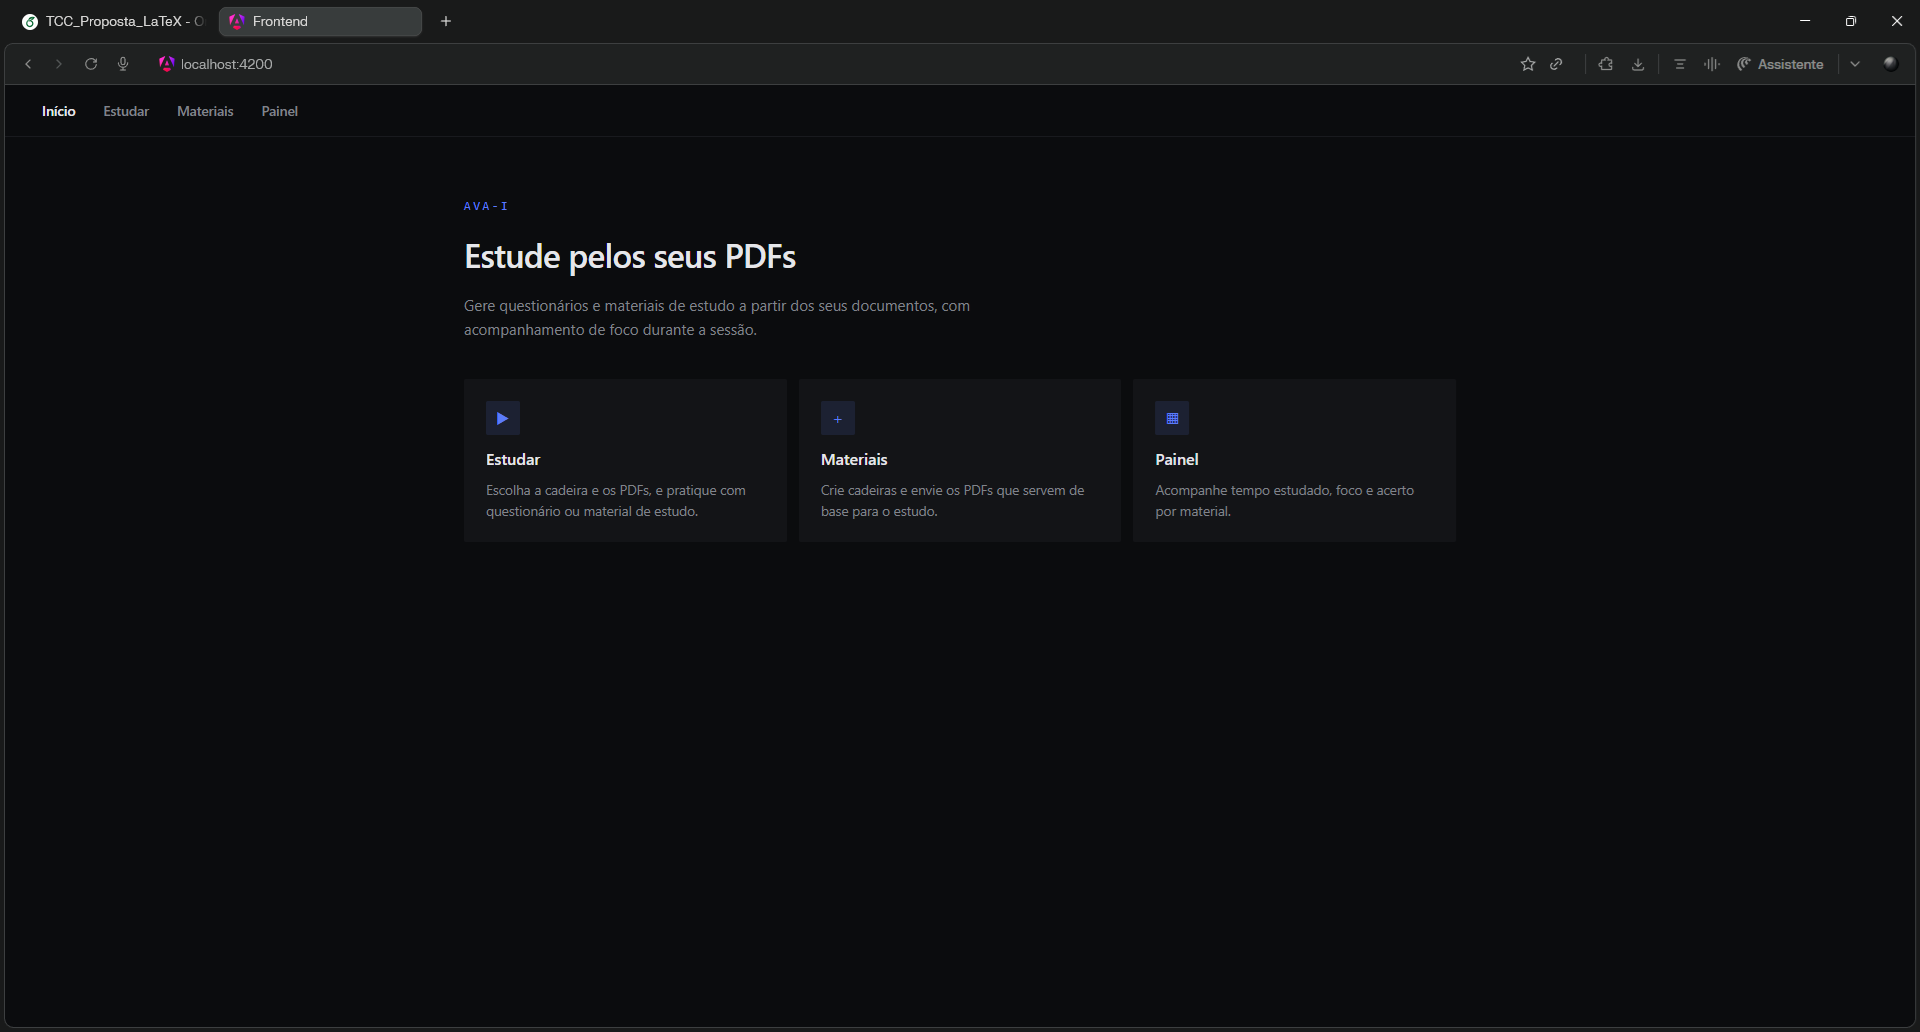
\includegraphics[width=0.9\textwidth]{lobby.png}
\caption{Tela inicial do AVA-I, com acesso aos módulos de estudo, materiais e painel.}
\label{fig:lobby}
\end{figure}

\textbf{Módulo 1: Geração de avaliações formativas (professor).} O professor envia os PDFs do material. O sistema fragmenta o texto, gera os \emph{embeddings}, indexa-os em um banco vetorial e, por RAG, usa esse conteúdo como fonte para o modelo de linguagem gerar perguntas formativas de múltipla escolha ancoradas em trechos específicos. O professor revisa, edita ou aprova cada questão e a publica, isto é, disponibiliza-a na própria plataforma para as sessões de estudo. A Figura~\ref{fig:materiais} mostra a gestão das cadeiras e dos materiais, com a pré-visualização de uma questão gerada a partir do PDF.

\begin{figure}[htbp]
\centering
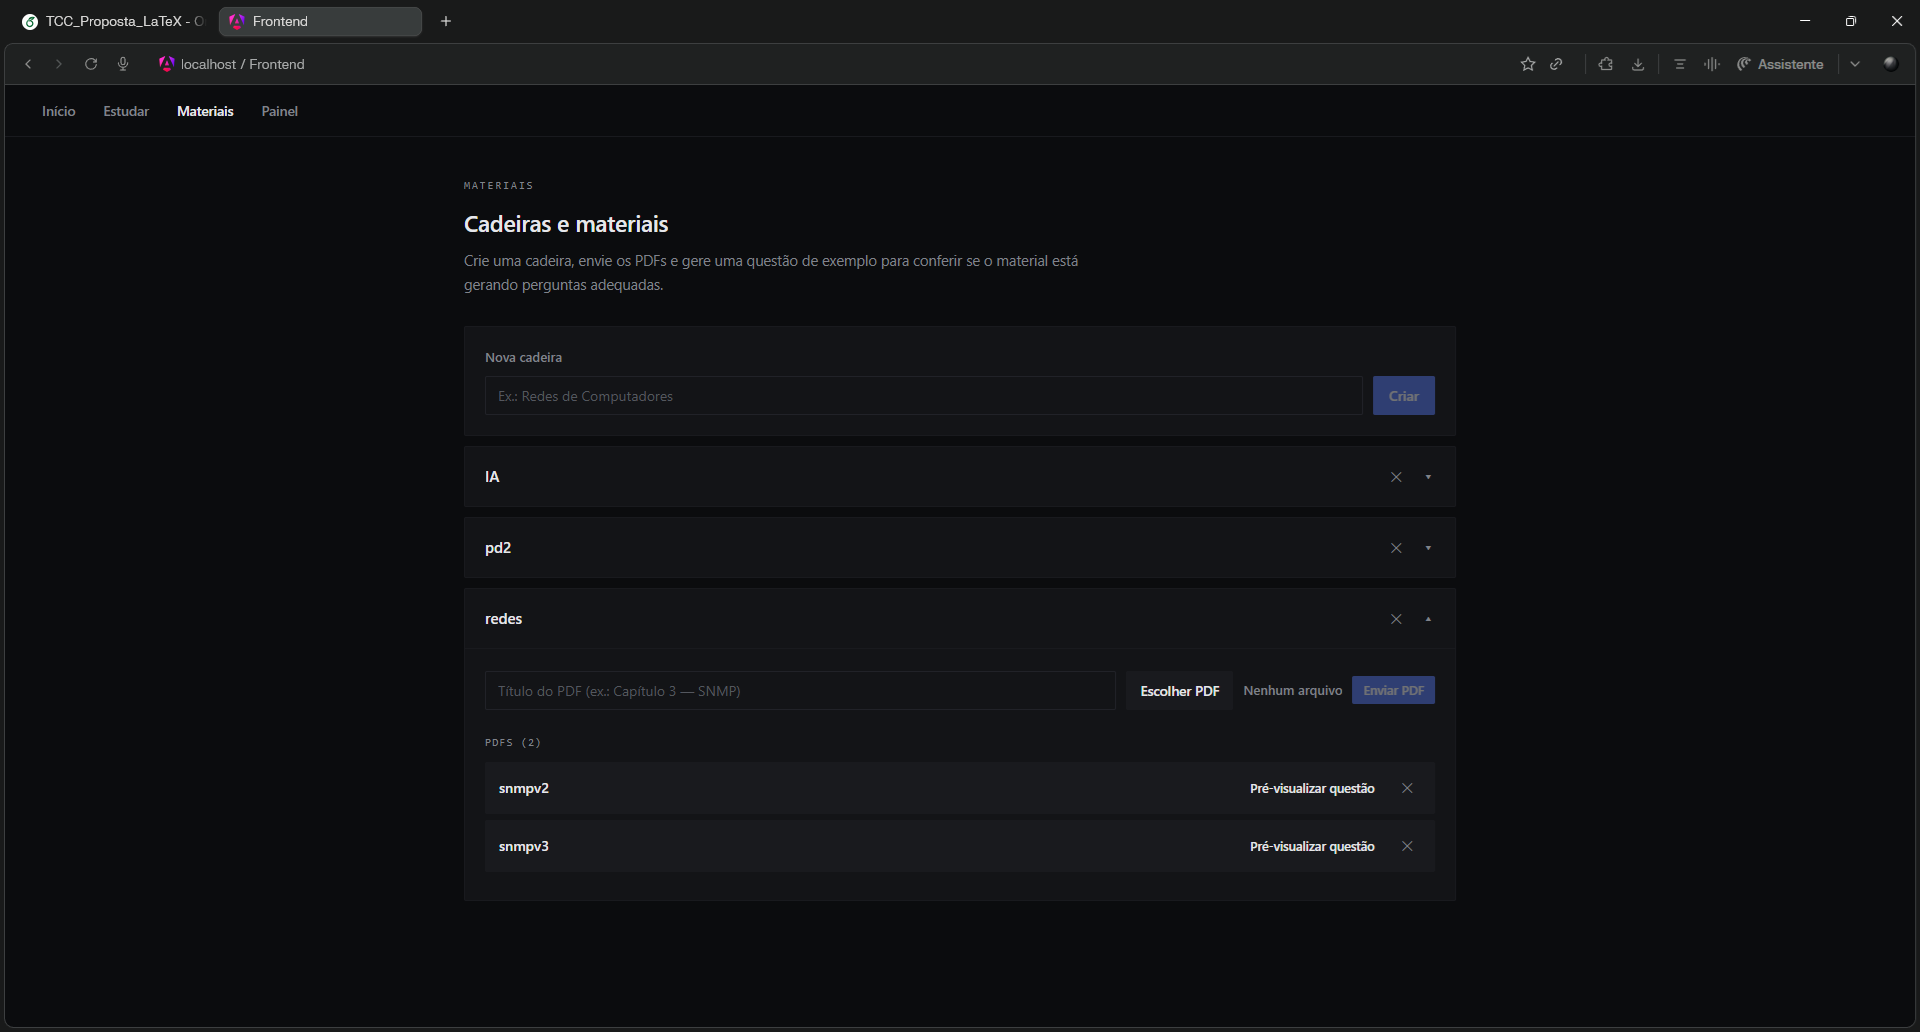
\includegraphics[width=0.9\textwidth]{materiais.png}
\caption{Módulo 1: gestão de cadeiras e materiais, com pré-visualização de uma questão gerada a partir do PDF enviado.}
\label{fig:materiais}
\end{figure}

\textbf{Módulo 2: Sessão de estudo inteligente (estudante).} O estudante lê o material dentro do AVA-I, e a leitura é intercalada com as perguntas do Módulo 1. Com consentimento prévio, a câmera é usada localmente, no navegador, para estimar os indicadores de engajamento (estado dos olhos, direção da cabeça e presença de \emph{smartphone}). Nenhum quadro de vídeo é enviado ao servidor; apenas as métricas agregadas são transmitidas. As Figuras~\ref{fig:selecao} a~\ref{fig:foco-estados} ilustram o fluxo do estudante: a seleção dos PDFs, uma questão com feedback imediato, a sessão de estudo com o indicador de foco e os estados reconhecidos pelo monitoramento.

\begin{figure}[htbp]
\centering
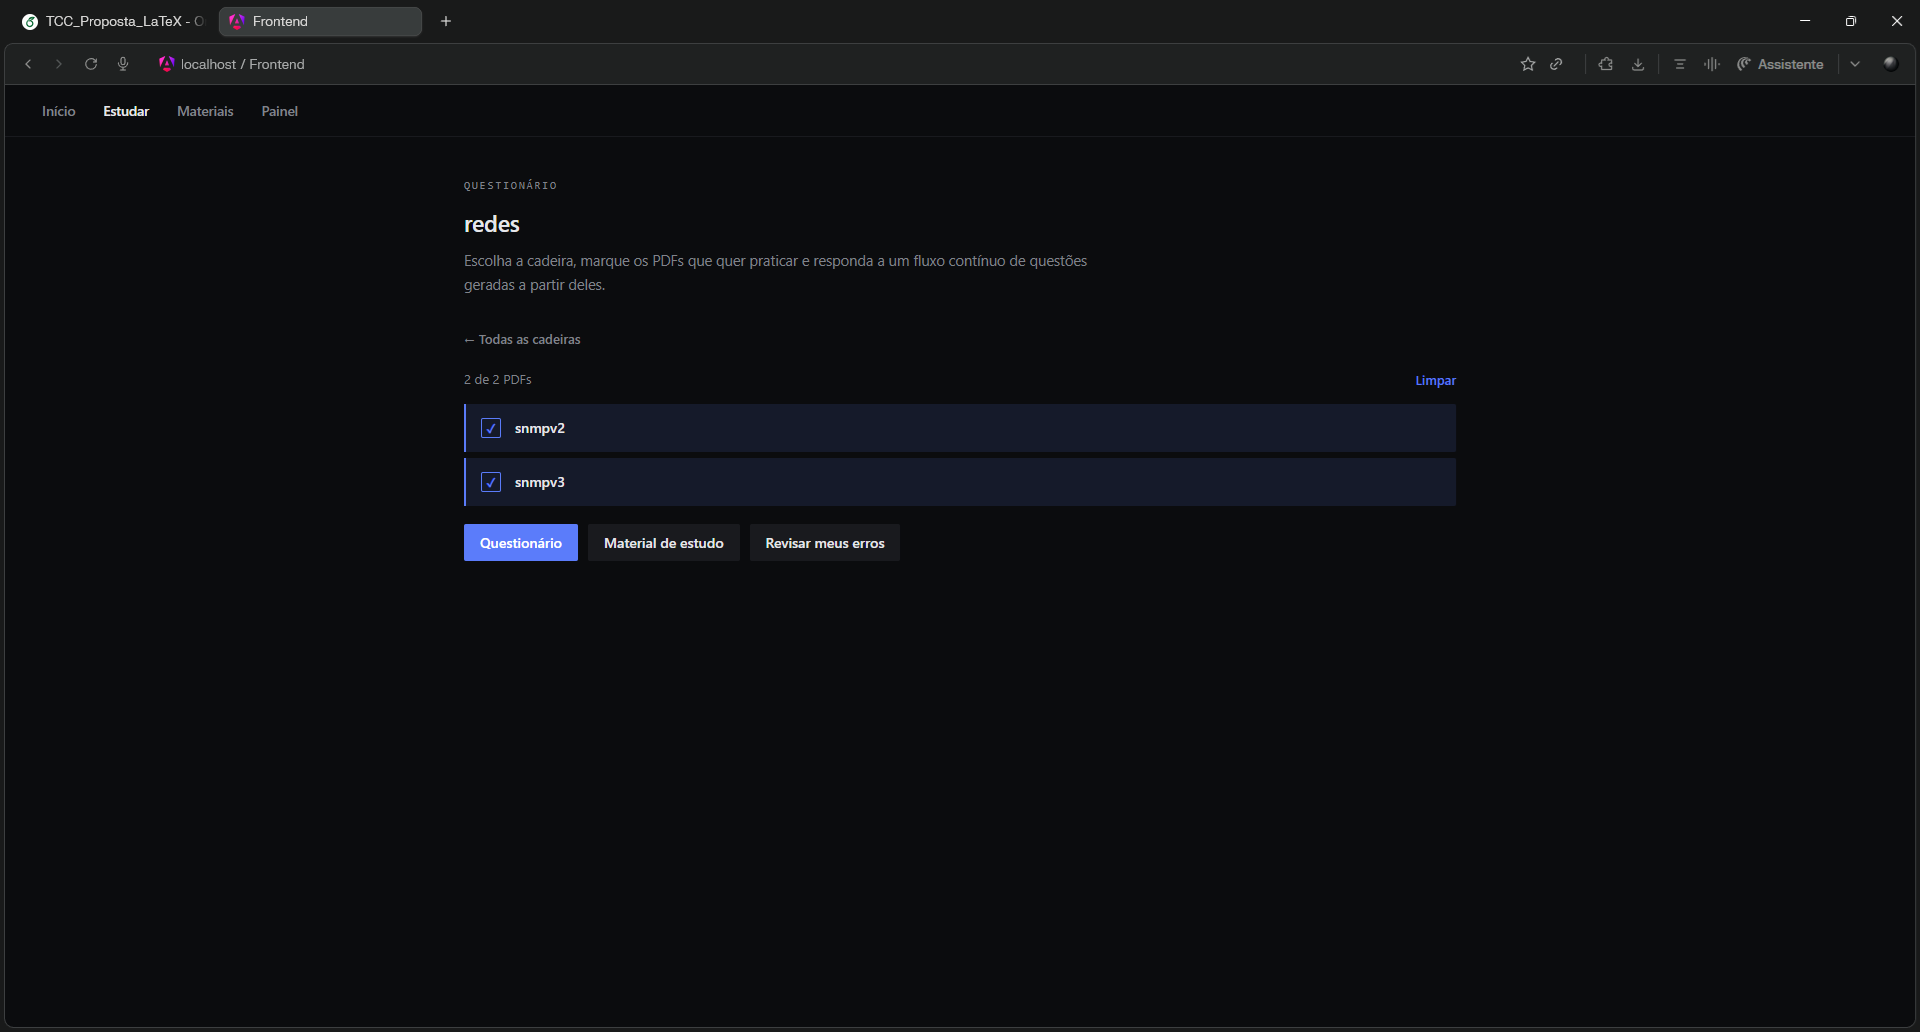
\includegraphics[width=0.9\textwidth]{selecao.png}
\caption{Módulo 2: seleção dos PDFs da cadeira e escolha entre questionário, material de estudo ou revisão dos erros.}
\label{fig:selecao}
\end{figure}

\begin{figure}[htbp]
\centering
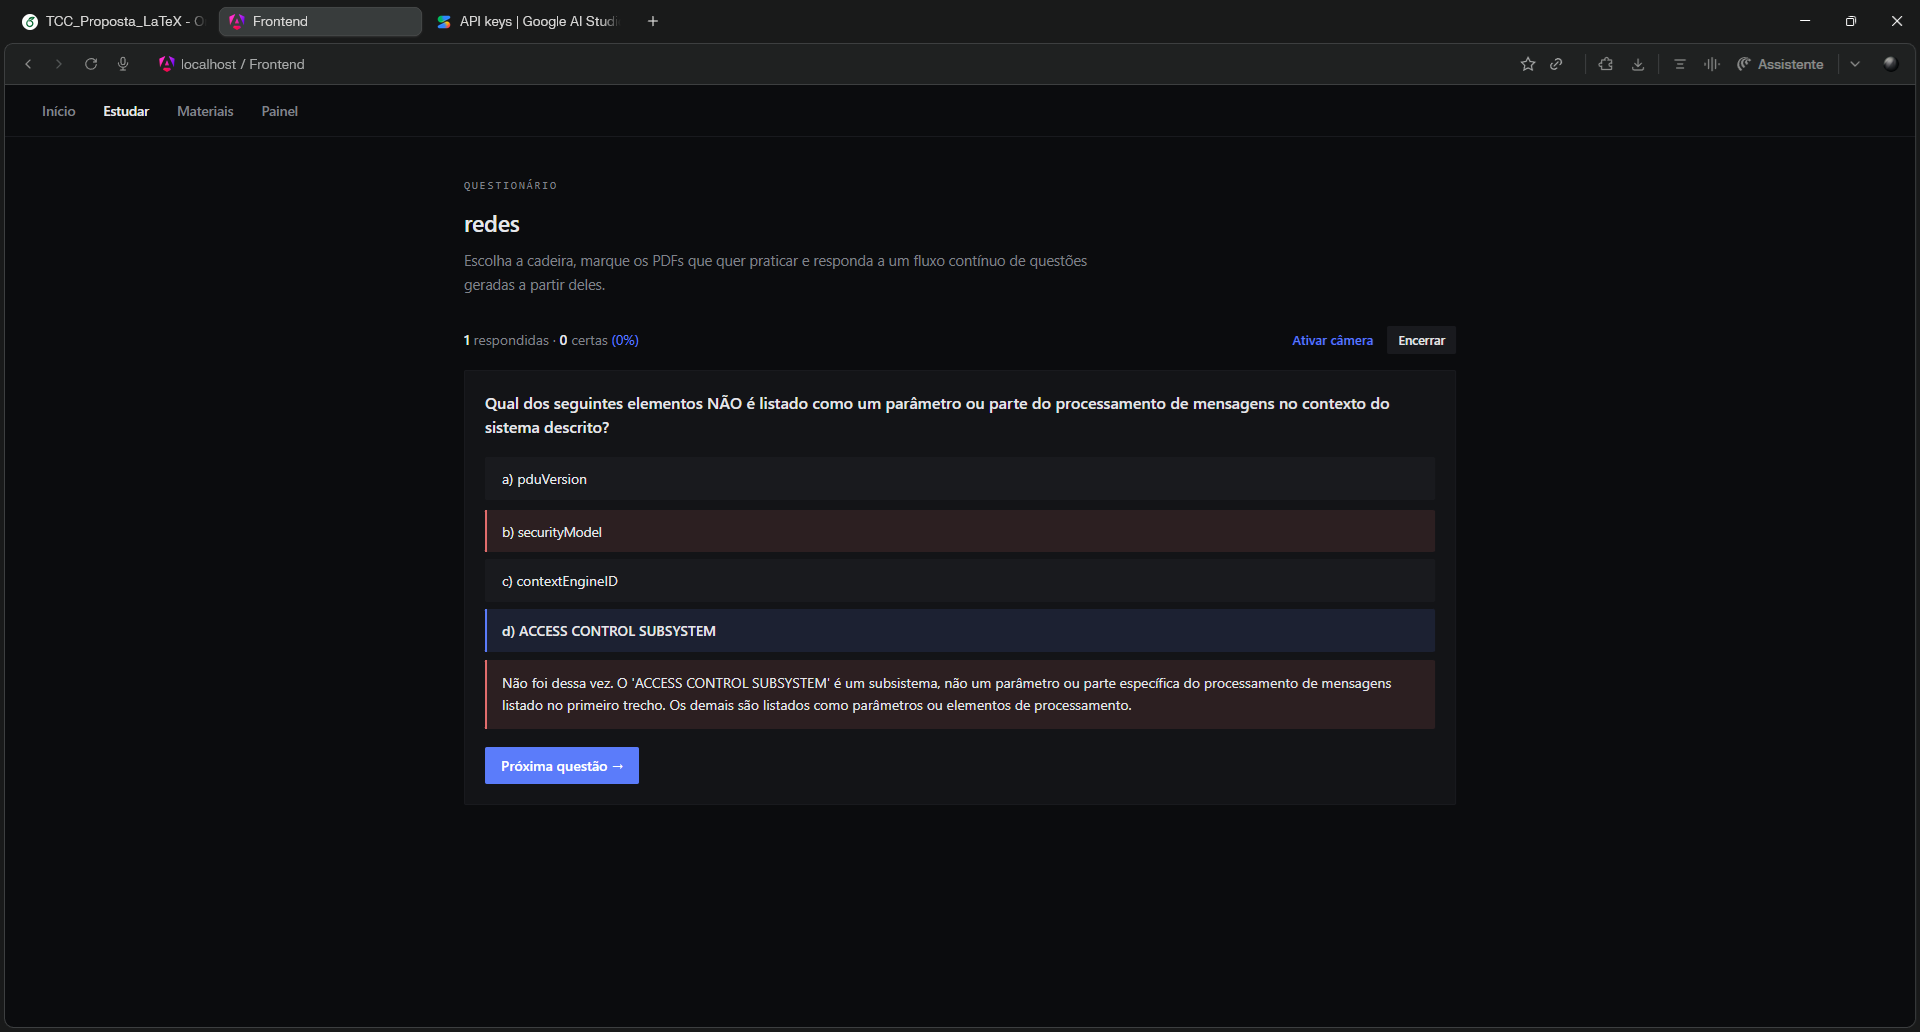
\includegraphics[width=0.9\textwidth]{quiz-feedback.png}
\caption{Módulo 2: questão formativa gerada a partir do material, com feedback imediato após a resposta.}
\label{fig:quiz}
\end{figure}

\begin{figure}[htbp]
\centering
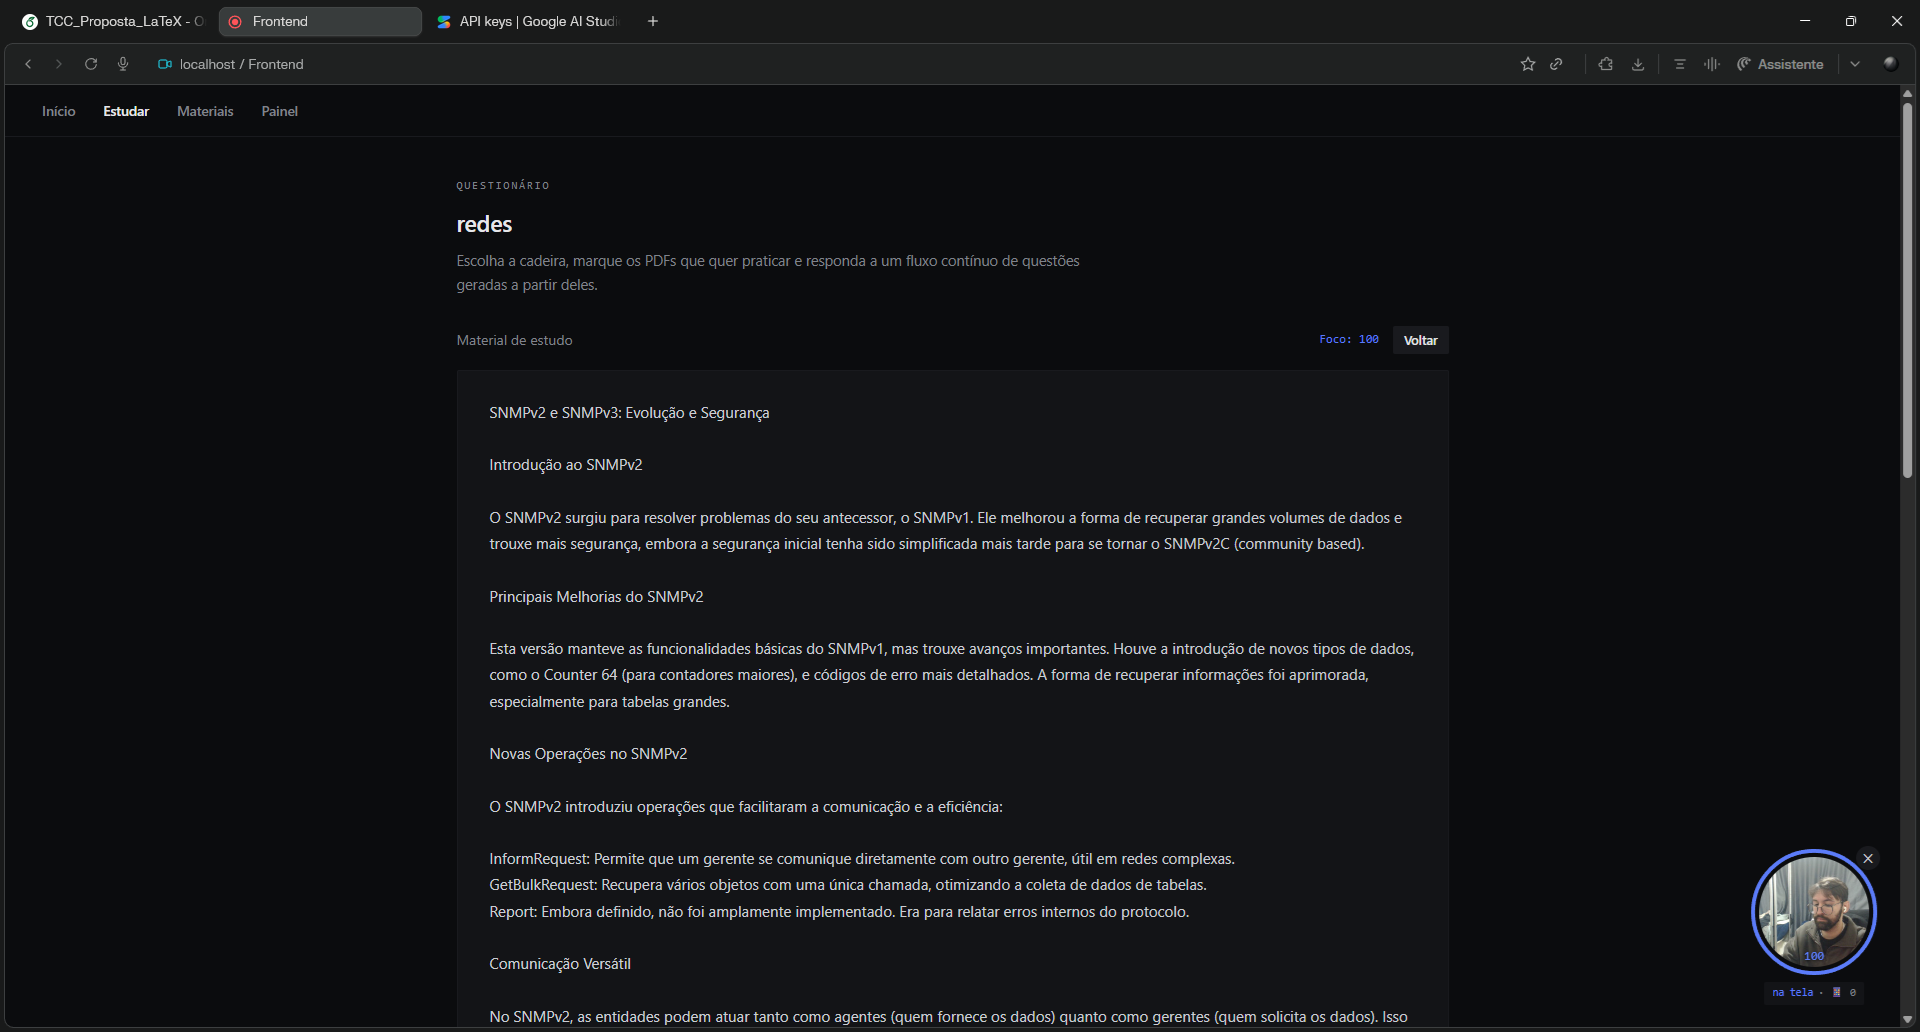
\includegraphics[width=0.9\textwidth]{estudo-foco.png}
\caption{Módulo 2: sessão de estudo com o indicador de foco (\emph{focusScore}). O processamento da câmera ocorre no navegador e a imagem não deixa o dispositivo.}
\label{fig:foco}
\end{figure}

\begin{figure}[htbp]
\centering
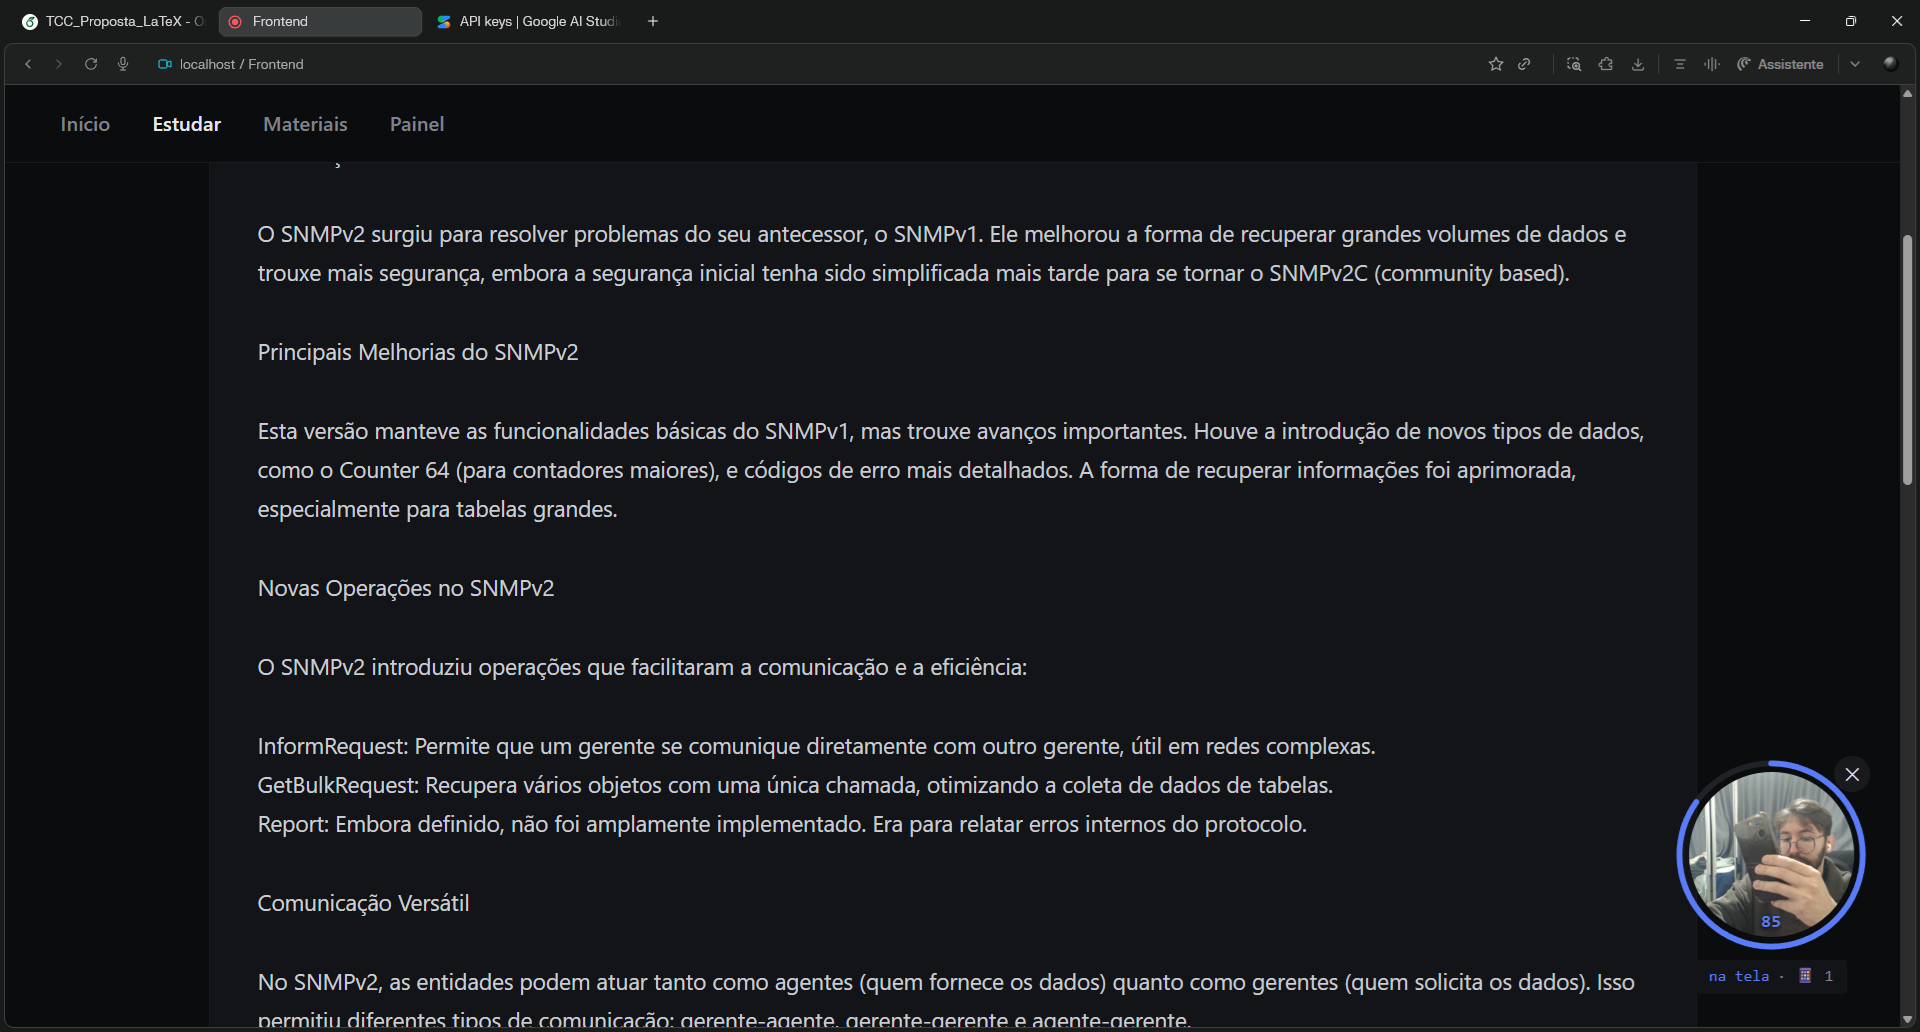
\includegraphics[width=0.48\textwidth]{foco-natela.png}\hfill
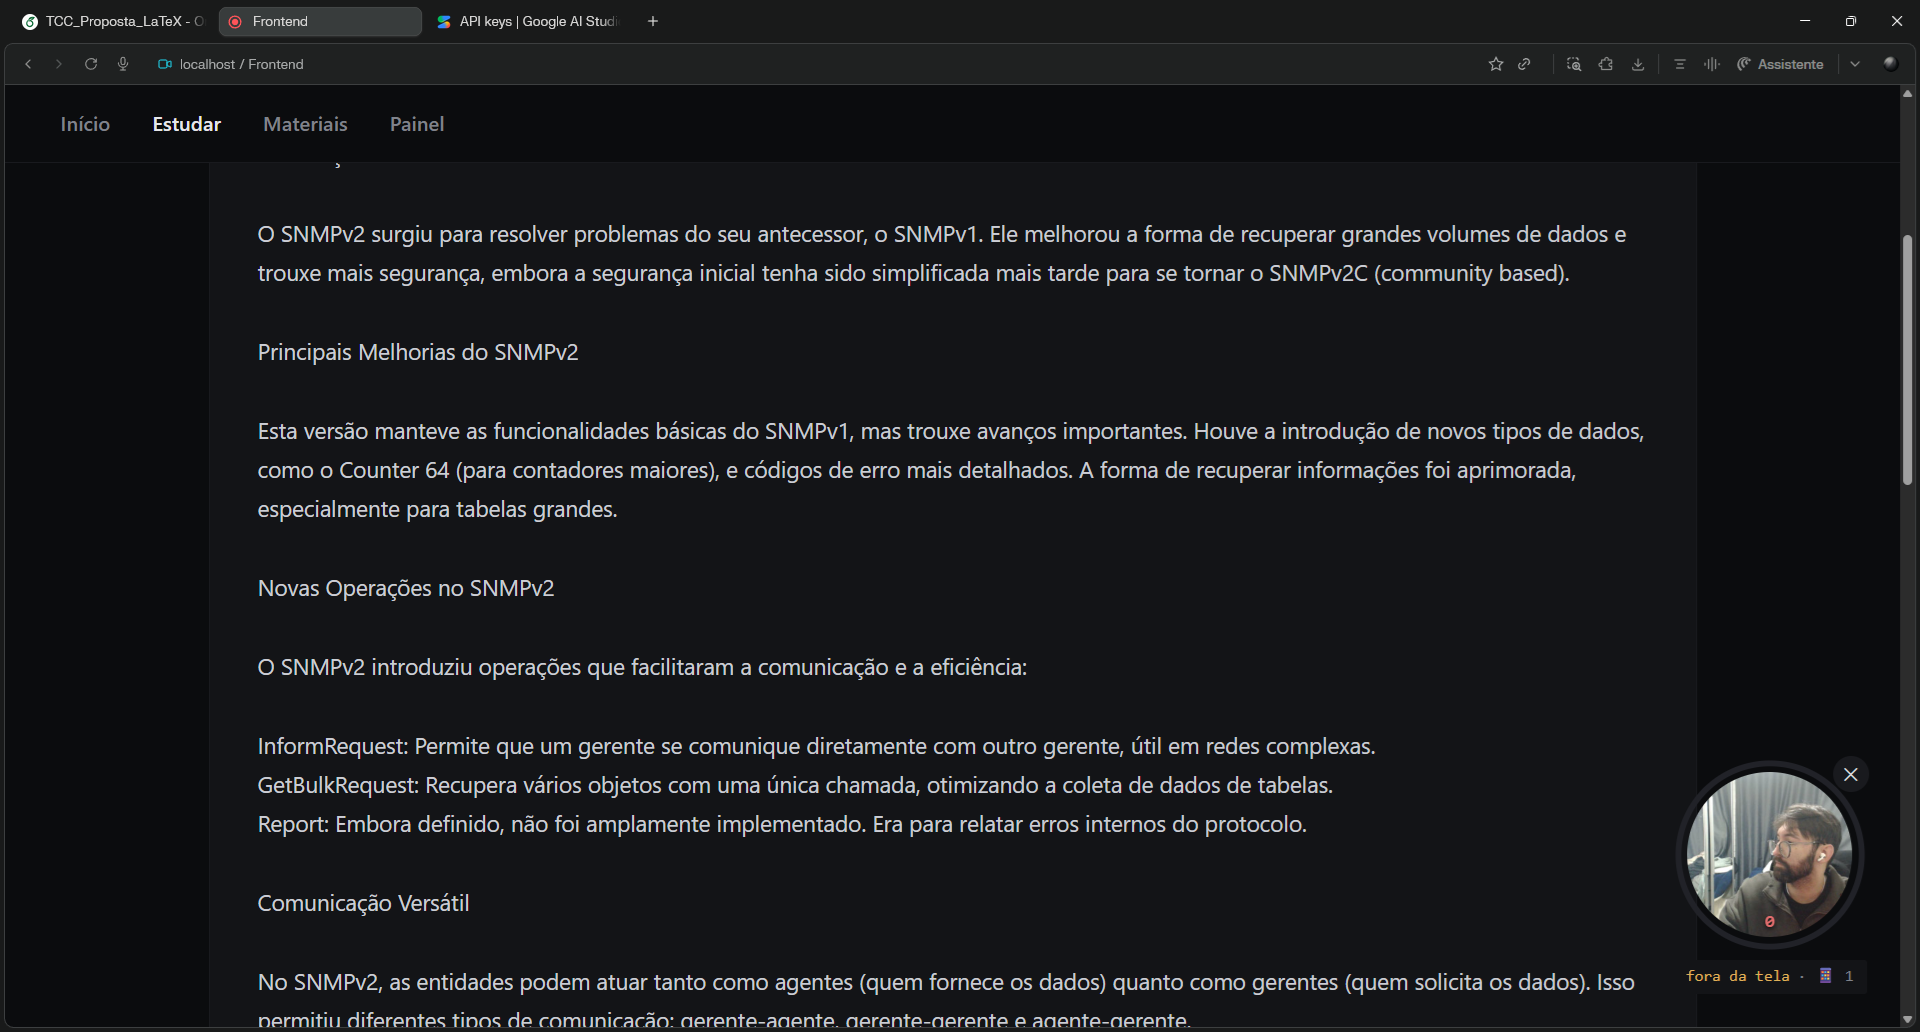
\includegraphics[width=0.48\textwidth]{foco-foratela.png}
\caption{Estados reconhecidos pelo monitoramento: à esquerda, atenção na tela com detecção de \emph{smartphone}; à direita, olhar fora da tela, com queda do indicador de foco.}
\label{fig:foco-estados}
\end{figure}

\textbf{Módulo 3: Painel analítico (professor).} De forma agregada e anonimizada, o professor visualiza em quais trechos a turma mais se dispersou, em quais perguntas houve mais erro e onde a queda de engajamento coincidiu com o baixo desempenho. Esses indícios ajudam o professor a revisar o próprio material. A Figura~\ref{fig:painel} mostra o painel, que reúne tempo estudado, foco médio, distrações com o celular, foco ao longo da sessão e acerto por material.

\begin{figure}[htbp]
\centering
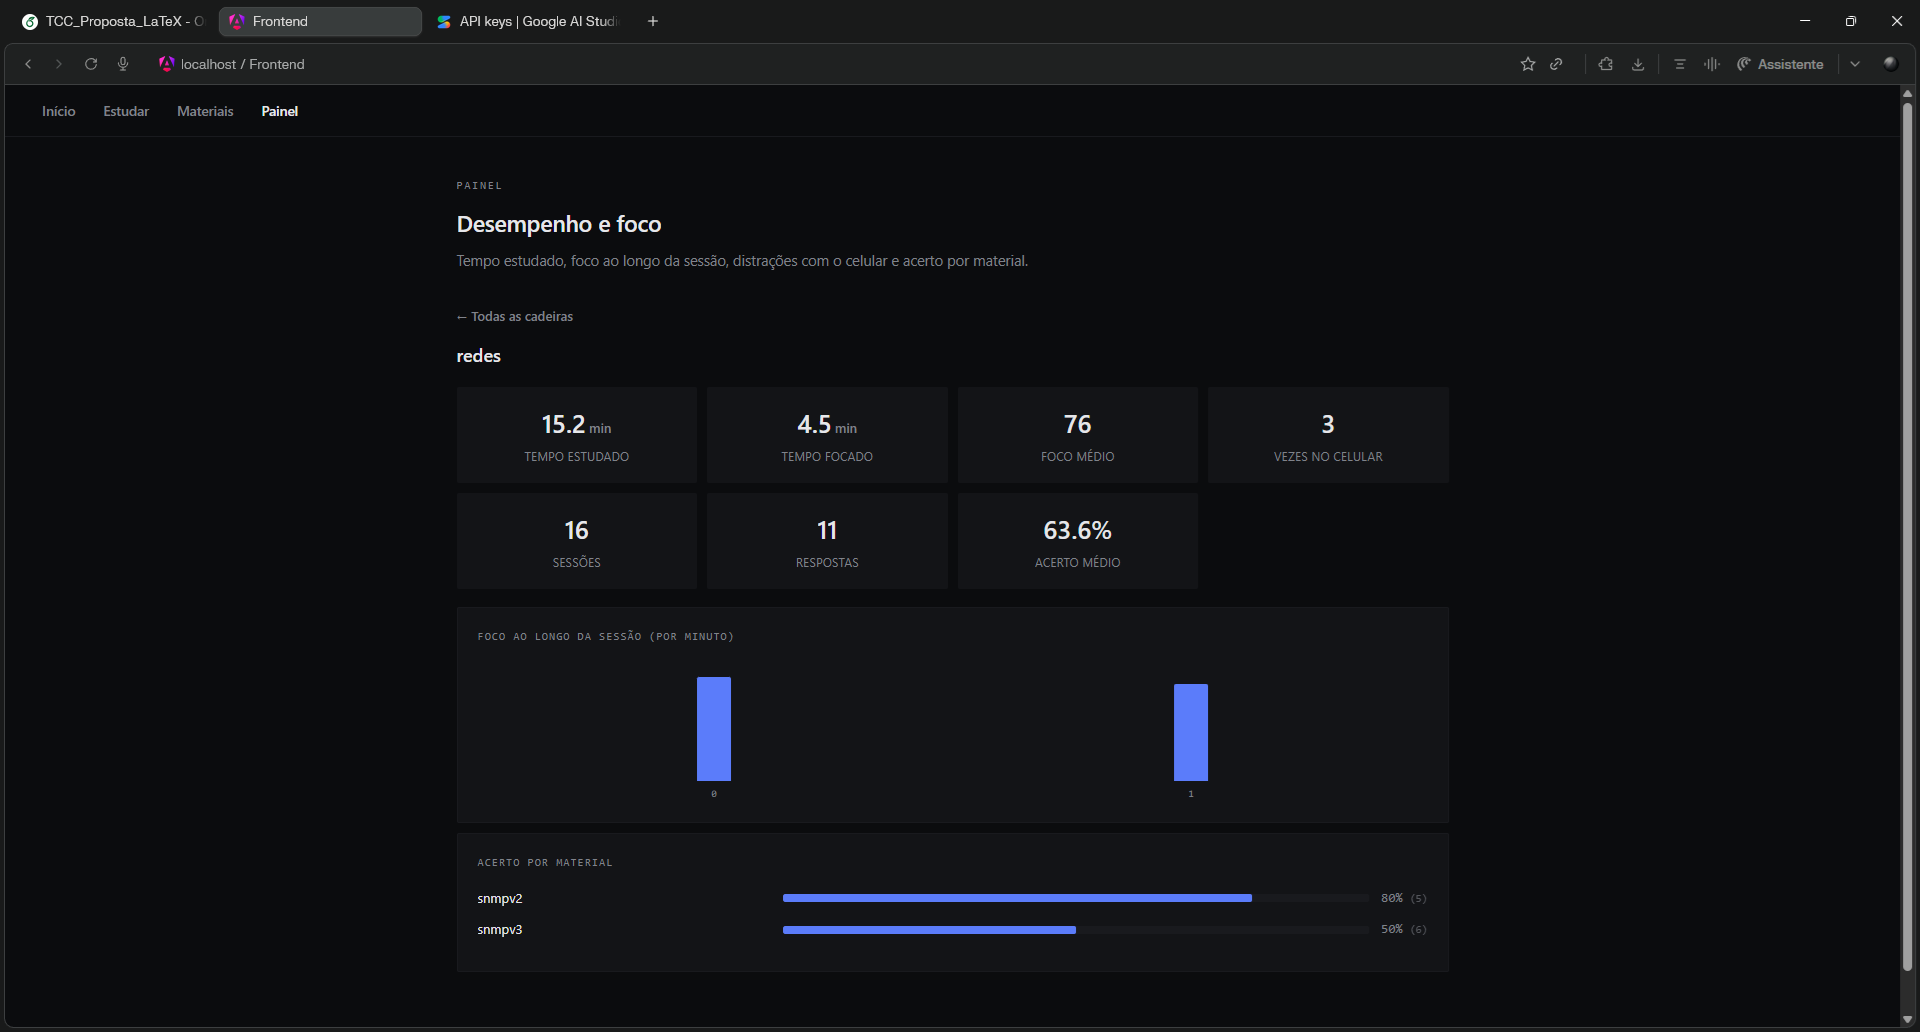
\includegraphics[width=0.9\textwidth]{painel.png}
\caption{Módulo 3: painel analítico que cruza engajamento (tempo, foco e distrações) com desempenho (acerto por material).}
\label{fig:painel}
\end{figure}

\subsection{Questões de pesquisa}

A avaliação (Capítulo~\ref{sec:aval}) é orientada por três questões de pesquisa.

\textbf{QP1: Engajamento e desempenho.} Existe relação entre o indicador agregado de engajamento visual e a taxa de acertos do estudante nas perguntas formativas geradas pela plataforma?

\textbf{QP2: Intervenção e dispersão.} Intercalar perguntas formativas durante a leitura reduz a frequência de uso do \emph{smartphone}, em comparação com a leitura do mesmo material sem essas perguntas? As perguntas não são geradas em tempo real durante a sessão: são geradas e revisadas pelo professor na fase de preparação, ficam armazenadas e são apresentadas em pontos de verificação predefinidos. Essa decisão também controla o custo de chamadas ao modelo.

\textbf{QP3: Usabilidade.} O processamento de visão computacional no navegador mantém a usabilidade da plataforma em nível aceitável? A usabilidade é medida pela \emph{System Usability Scale} (SUS) \cite{Bro96}, questionário padronizado de 0 a 100; valores em torno de 68 são tomados como limiar de aceitabilidade conforme Bangor et al. \cite{BKM08}.

% ===========================================================================
\section{Arquitetura e Integração Tecnológica}\label{sec:arq}

A plataforma é organizada em três camadas. O critério arquitetural central é o \emph{privacy by design} discutido na Seção~\ref{sub:priv} \cite{HBF19,UNE21}: o processamento de imagem ocorre integralmente no cliente, e a rede transporta apenas dados agregados.

\subsection{\emph{Frontend}: Single Page Application}

O \emph{frontend} é uma \emph{Single Page Application} (SPA), aplicação web que carrega uma única vez e atualiza o conteúdo sem recarregar a página, construída em Angular com TypeScript. Sobre essa base rodam dois modelos de visão computacional:

\begin{itemize}[leftmargin=*]
  \item \textbf{MediaPipe Face Mesh} \cite{LTN19,KAGG19}, para extrair os pontos faciais em tempo real. Sobre eles, o cliente calcula o EAR \cite{SC16} e estima a direção da cabeça, e deriva o indicador de engajamento (\emph{focusScore}), definido como a proporção do tempo, em uma janela de observação, em que (i) o rosto é detectado, (ii) a cabeça está voltada para a tela e (iii) o EAR está acima de um limiar calibrado para cada usuário, em uma calibração no início da sessão.
  \item \textbf{YOLOv8-nano} \cite{RDGF16,JCQ23}, exportado para o formato ONNX (um padrão aberto que permite executar modelos já treinados em diferentes ambientes, inclusive no navegador) e executado no navegador, para detectar a classe \emph{smartphone} no campo da câmera. Cada detecção registra um evento associado ao instante da sessão.
\end{itemize}

\subsubsection{Tratamento explícito da limitação de \emph{hardware}}\label{sub:hw}

A inferência do YOLO no navegador é sensível ao \emph{hardware} do cliente \cite{JCQ23}. Para lidar com isso, a SPA verifica, ao carregar, se o modelo inicializa e responde em tempo útil; caso o navegador não disponha de aceleração gráfica funcional ou a inferência não seja viável, o módulo de detecção de \emph{smartphone} é desligado de forma graciosa, e a sessão segue apenas com os indicadores faciais, mais leves. Esse modo degradado fica registrado nos metadados da sessão: sessões em modo degradado não entram na verificação da QP2.

\subsection{\emph{Backend}: API REST}

O \emph{backend} é construído em Python com FastAPI, escolhido pelo desempenho em entrada e saída assíncrona e pela validação de dados nativa, úteis para orquestrar chamadas a modelos de linguagem com latência variável. Suas responsabilidades são: gestão de sessões; recebimento da telemetria agregada (as métricas numéricas resumidas da sessão, como o foco e a contagem de eventos), nunca de fluxos de vídeo; orquestração das chamadas ao módulo de RAG; persistência dos materiais, sessões e respostas; e entrega dos dados consolidados ao painel.

\subsection{Módulo de IA generativa (RAG)}

O módulo de RAG é implementado em Python. Os PDFs do professor passam por extração de texto, fragmentação em \emph{chunks} de tamanho configurável e geração de \emph{embeddings} com modelos abertos. Os vetores são indexados em um banco vetorial (ChromaDB), e a geração das perguntas fica a cargo de um modelo de linguagem acessado por API, condicionado ao contexto recuperado \cite{LPP20,GXG23}. Cabe um cuidado de escala: o índice cresce com a quantidade e o tamanho dos PDFs, e um \emph{corpus} muito grande pode tornar a indexação e a busca custosas; por isso, o índice é organizado por disciplina e, no escopo da PoC, o \emph{corpus} é delimitado.

\subsection{Fluxo de dados}

\begin{enumerate}[leftmargin=*]
  \item O professor envia o PDF; o \emph{backend} aciona a ingestão e indexa o conteúdo.
  \item O estudante inicia a sessão; a SPA roda sempre o Face Mesh e tenta rodar o YOLO, se viável.
  \item A cada poucos segundos, a SPA envia ao \emph{backend} um lote com o instante, o \emph{focusScore}, a contagem de eventos de \emph{smartphone} e o modo da sessão.
  \item Em cada ponto de verificação, uma pergunta previamente gerada é apresentada; a resposta do aluno volta para o \emph{backend}.
  \item O painel consulta o \emph{backend} para cruzar engajamento e desempenho.
\end{enumerate}

% ===========================================================================
\section{Metodologia}\label{sec:met}

A pesquisa é aplicada, de abordagem quantitativa-qualitativa, e segue a \emph{Design Science Research} (DSR) \cite{HMPR04}, metodologia voltada a resolver problemas reais por meio da construção e da avaliação de um artefato. Aqui, o artefato é um protótipo funcional do AVA-I; construí-lo e avaliá-lo é o que gera o conhecimento pretendido sobre a viabilidade e os limites da abordagem. O desenvolvimento está organizado em quatro fases, e cada componente é avaliado de forma independente antes da avaliação integrada com usuários.

\subsection{Fase 1: Revisão complementar e especificação}
Aprofundamento do referencial em três frentes: ITS com LLMs (com foco em trabalhos posteriores a VanLehn \cite{Van11}); medição automática de engajamento \cite{DDD17,AK24,DD25}; e aspectos legais \cite{Bra18}. Ao fim da fase, a especificação técnica é congelada.

\subsection{Fase 2: \emph{Backend} e \emph{pipeline} RAG}
Construção da API em FastAPI, modelagem do banco e implementação do \emph{pipeline} de RAG com ChromaDB. A validação interna gera questões para três materiais de referência (capítulos de livros-texto abertos), com inspeção manual da qualidade pelos autores e revisão do orientador.

\subsection{Fase 3: \emph{Frontend} e módulos de VC}
Desenvolvimento da SPA em Angular e integração do MediaPipe Face Mesh e do YOLOv8-nano. O MediaPipe é escolhido pela maturidade no navegador e pelo custo computacional baixo, recorrente em estudos de engajamento \cite{LTN19,AK24,DD25}; o YOLOv8-nano, pelo equilíbrio entre acurácia e latência no cliente, com a ressalva de \emph{hardware} já discutida \cite{JCQ23}. Os limiares de EAR e de direção da cabeça são calibrados em um piloto interno, usado apenas para ajustar parâmetros, não para validar as questões de pesquisa.

\subsection{Fase 4: Avaliação experimental controlada}
Execução do protocolo do Capítulo~\ref{sec:aval}, com aprovação prévia do CEP-PUCRS. A coleta ocorre fora do horário de aula, no ambiente doméstico do estudante, com sessões guiadas remotamente.

% ===========================================================================
\section{Avaliação}\label{sec:aval}

\subsection{Considerações éticas}
Por envolver coleta de dados com seres humanos (estudantes voluntários, com captura de imagem, ainda que processada localmente), o projeto será submetido ao CEP-PUCRS, via Plataforma Brasil, antes de qualquer coleta. Estão previstos: protocolo de pesquisa, Termo de Consentimento Livre e Esclarecido (TCLE), descrição das medidas de minimização de risco (nenhum vídeo trafega pela rede; apenas métricas agregadas são armazenadas) e plano de descarte dos dados. A submissão ao CEP é condição para iniciar a Fase 4.

\subsection{Desenho experimental}
A avaliação usa um desenho intra-sujeitos: cada participante passa pelas duas condições e serve como seu próprio controle. A ordem das condições é contrabalanceada para diluir efeitos de ordem, aprendizagem e fadiga \cite{WRH12}.

\begin{itemize}[leftmargin=*]
  \item \textbf{Condição A (controle):} leitura do material no AVA-I sem as perguntas formativas. A telemetria de engajamento roda em segundo plano.
  \item \textbf{Condição B (intervenção):} leitura de material equivalente (pareado em tamanho e dificuldade), com perguntas formativas inseridas nos pontos de verificação. Telemetria igual à da condição A.
\end{itemize}

Cada participante faz as duas sessões com pelo menos 24 horas de intervalo, em ordem aleatória e com materiais distintos. Cada sessão dura de 30 a 40 minutos. O desenho intra-sujeitos decorre do tamanho da amostra: comparar cada pessoa consigo mesma elimina a variabilidade entre indivíduos e isola melhor o efeito da intervenção, o que aumenta o poder estatístico; Wohlin et al. \cite{WRH12} recomendam esse arranjo quando o número de participantes é limitado.

\subsection{Participantes}
De 12 a 18 estudantes voluntários de Ciência da Computação ou áreas afins da PUCRS, maiores de 18 anos, com acesso a \emph{notebook} com câmera. O intervalo amostral considera o caráter exploratório do estudo, a literatura de testes de usabilidade \cite{Nie00} (os ganhos em descoberta de problemas decrescem após cerca de 15 participantes) e a heterogeneidade de \emph{hardware}, que deve reduzir as sessões válidas para a QP2.

\subsection{Indicadores}
A plataforma extrai três indicadores quantitativos, fundamentados na literatura:
\begin{itemize}[leftmargin=*]
  \item \textbf{Engajamento visual (\emph{focusScore}):} proporção do tempo com rosto detectado, cabeça voltada para a tela e EAR acima do limiar individual, baseado no EAR de Soukupová e Cech \cite{SC16} e no arcabouço de medição de engajamento de D'Mello et al. \cite{DDD17}.
  \item \textbf{Eventos de \emph{smartphone}:} número de intervalos em que a classe \emph{smartphone} foi detectada por pelo menos $k$ quadros consecutivos. Aplicável apenas a sessões fora do modo degradado.
  \item \textbf{Taxa de acertos:} proporção de acertos nas perguntas formativas (condição B). Cada pergunta é revisada pelos autores e pelo orientador antes da sessão.
\end{itemize}
Coleta-se ainda a usabilidade pela SUS \cite{Bro96}, interpretada conforme Bangor et al. \cite{BKM08}.

\subsection{Análise estatística}
A escolha dos testes depende do tamanho da amostra. Testes paramétricos clássicos, como o teste $t$ e a correlação de Pearson, pressupõem que os dados seguem uma distribuição normal, isto é, concentrada em torno da média e simétrica. Com a amostra prevista ($n \leq 18$), esse pressuposto não pode ser verificado de forma confiável, e um único valor atípico já distorceria o resultado, o que torna tais testes inadequados \cite{Fie13}. Por isso, adotam-se testes não paramétricos, que trabalham com a ordem (o \emph{ranking}) dos valores em vez dos valores brutos e, portanto, não exigem normalidade e toleram melhor amostras pequenas. Na prática, a correlação de Pearson é substituída pela de Spearman e o teste $t$ pelo de Wilcoxon:
\begin{itemize}[leftmargin=*]
  \item \textbf{QP1:} correlação de Spearman entre o \emph{focusScore} e a taxa de acertos na condição B. A correlação de Spearman mede se duas grandezas tendem a subir ou descer juntas, comparando a ordem (o \emph{ranking}) dos valores em vez dos valores brutos, e varia de $-1$ (relação inversa perfeita) a $+1$ (relação direta perfeita). Reportam-se o coeficiente, o $p$-valor (probabilidade de obter um resultado igual ou mais forte por acaso, caso não houvesse relação real) e o intervalo de confiança estimado por \emph{bootstrap}, técnica que reamostra os próprios dados muitas vezes para medir a incerteza sem supor normalidade.
  \item \textbf{QP2:} teste de Wilcoxon dos postos sinalizados, a versão não paramétrica do teste $t$ para dados pareados, que compara as duas medidas de um mesmo participante a partir da ordem das diferenças entre elas. Compara os eventos de \emph{smartphone} de cada participante nas condições A e B, considerando apenas as sessões fora do modo degradado, e reporta a estatística do teste, o $p$-valor e o tamanho do efeito (uma medida de quão grande é a diferença, e não apenas se ela existe).
  \item \textbf{QP3:} estatística descritiva (média, mediana e dispersão) das notas da SUS, comparada aos parâmetros de referência de Bangor et al. \cite{BKM08}.
\end{itemize}
Os resultados são reportados com a ressalva de que o estudo é exploratório: o objetivo é gerar evidência preliminar sobre a viabilidade, não generalizar para a população.

\subsection{Avaliação do painel pelo docente}
Em paralelo à avaliação com estudantes, o painel passa por uma avaliação qualitativa própria:
\begin{itemize}[leftmargin=*]
  \item \textbf{Inspeção heurística} com 2 a 3 docentes, usando as heurísticas de Nielsen \cite{Nie94}, um conjunto de dez princípios consagrados de boa usabilidade (como manter o usuário informado do estado do sistema e prevenir erros), aplicados para encontrar problemas de interface e de clareza analítica.
  \item \textbf{Entrevista semiestruturada} com cada docente, após usar o painel com dados anonimizados de uma turma simulada, abordando clareza dos indicadores, utilidade para revisar o material, confiança nas perguntas geradas e intenção de uso futuro.
  \item \textbf{Análise de conteúdo} das entrevistas, segundo Bardin \cite{Bar11}, com codificação por dois autores e consenso por triangulação.
\end{itemize}
Essa etapa responde diretamente à pergunta de como saber se a plataforma é útil para o professor.

% ===========================================================================
\section{Considerações Finais}

Esta proposta reúne, em uma única plataforma, a geração automática de avaliações formativas por RAG, a medição local de engajamento por visão computacional e um painel analítico para o professor. A privacidade é tratada por arquitetura, com todo o processamento de imagem no navegador, e não como política acessória \cite{HBF19,UNE21}. As escolhas técnicas se apoiam no referencial do Capítulo~\ref{sec:ref} e, onde há restrições reais, como o custo de rodar o YOLO no navegador \cite{JCQ23}, a proposta as reconhece e prevê um caminho de degradação graciosa.

É preciso registrar uma limitação do próprio indicador: o \emph{focusScore} mede ``olhar para a tela com os olhos abertos e a cabeça na direção certa'', que é um \emph{proxy} de atenção, não a atenção em si. O sistema não distingue leitura concentrada de divagação com os olhos na tela; por isso o termo adotado é ``engajamento visual''. A avaliação (Capítulo~\ref{sec:aval}) combina métodos quantitativos não paramétricos, adequados ao tamanho da amostra, com métodos qualitativos junto a docentes, e está condicionada à aprovação do Comitê de Ética em Pesquisa.

Ao final, espera-se contribuir com (i) evidência preliminar sobre a relação entre engajamento visual e desempenho em avaliações geradas por IA; (ii) uma discussão fundamentada sobre os limites práticos de rodar modelos de aprendizado profundo no navegador para monitoramento educacional com privacidade preservada; e (iii) um artefato funcional que sirva de base para trabalhos futuros em AVAs inteligentes.

% ===========================================================================
\bibliographystyle{alpha}
\bibliography{tcc-bib}

\end{document}
